\chapter{冰、水、水蒸气}\label{ch:g2:ice-water-steam}

同一种水，在杯中以冰块的形式发出叮当声，
倒出来便是饮料，从汤锅里升起时便成为白色水汽。同一种物质，
却有\emph{三种状态}。去年我们看到热量使冰块熔化；
今年我们将认识水能够呈现的三种物质状态。

\section{水的三种状态}

\begin{example}[各种状态出现在哪里]\label{ex:g2:ice-water-steam:where}
水可以处于三种\emph{物质状态}。\emph{固体}：冰 ---
冰块、屋檐下的冰柱、草地上的霜、雪。固体是
坚硬的，能保持自己的形状。\emph{液体}：倒出来的水 ---
雨水、河流、大海，还有你杯中的水。液体会流动，
并取杯子的形状。\emph{气体}：水蒸气，看不见地
在空气中飘动。固体、液体、气体——底下始终是同一种物质。
\end{example}

\begin{omfigure}
\begin{tikzpicture}[scale=0.85]
  \draw[thick, omDef] (0.3,0.1) rectangle (1.5,1.3);
  \node[below, font=\small] at (0.9,-0.2) {冰：固体};
  \draw[thick] (3.9,1.5) -- (4.2,0.1) -- (5.6,0.1) -- (5.9,1.5);
  \fill[omDef, opacity=0.25] (4.13,0.45) -- (5.67,0.45)
    -- (5.75,1.1) -- (4.05,1.1) -- cycle;
  \node[below, font=\small] at (4.9,-0.2) {水：液体};
  \draw[thick] (8.0,0.1) rectangle (10.4,1.0);
  \draw[thick] (10.4,0.75) -- (11.0,0.85);
  \foreach \x/\y in {8.6/1.35, 9.2/1.7, 9.8/1.4, 9.0/2.05} {
    \draw[omExo, thick] (\x,\y) circle (0.22);
  }
  \node[below, font=\small] at (9.2,-0.2) {水蒸气：气体};
\end{tikzpicture}

{\small 同一种物质的三种状态：固体冰块、
一杯液体，以及锅上方显示出气体存在的水汽。}
\end{omfigure}

\begin{remark}[水蒸气是看不见的]\label{rem:g2:ice-water-steam:invisible}
你在锅上方看到的白色水汽，是由许多细小的漂浮
水滴构成的，也就是\emph{液体}的小水珠。真正的气体——
混入空气中的水蒸气——根本看不见！仔细观察
锅嘴：就在它的正上方，有一小段\emph{透明}的空隙，
然后白色水汽才开始出现。在这段空隙中，水是气体，
看不见；再往上一点，它聚集成我们能看到的小水滴。
每个房间的空气中都藏着看不见的水蒸气，我们
在本章结束前就能把它当场抓住。
\end{remark}

\begin{omfigure}
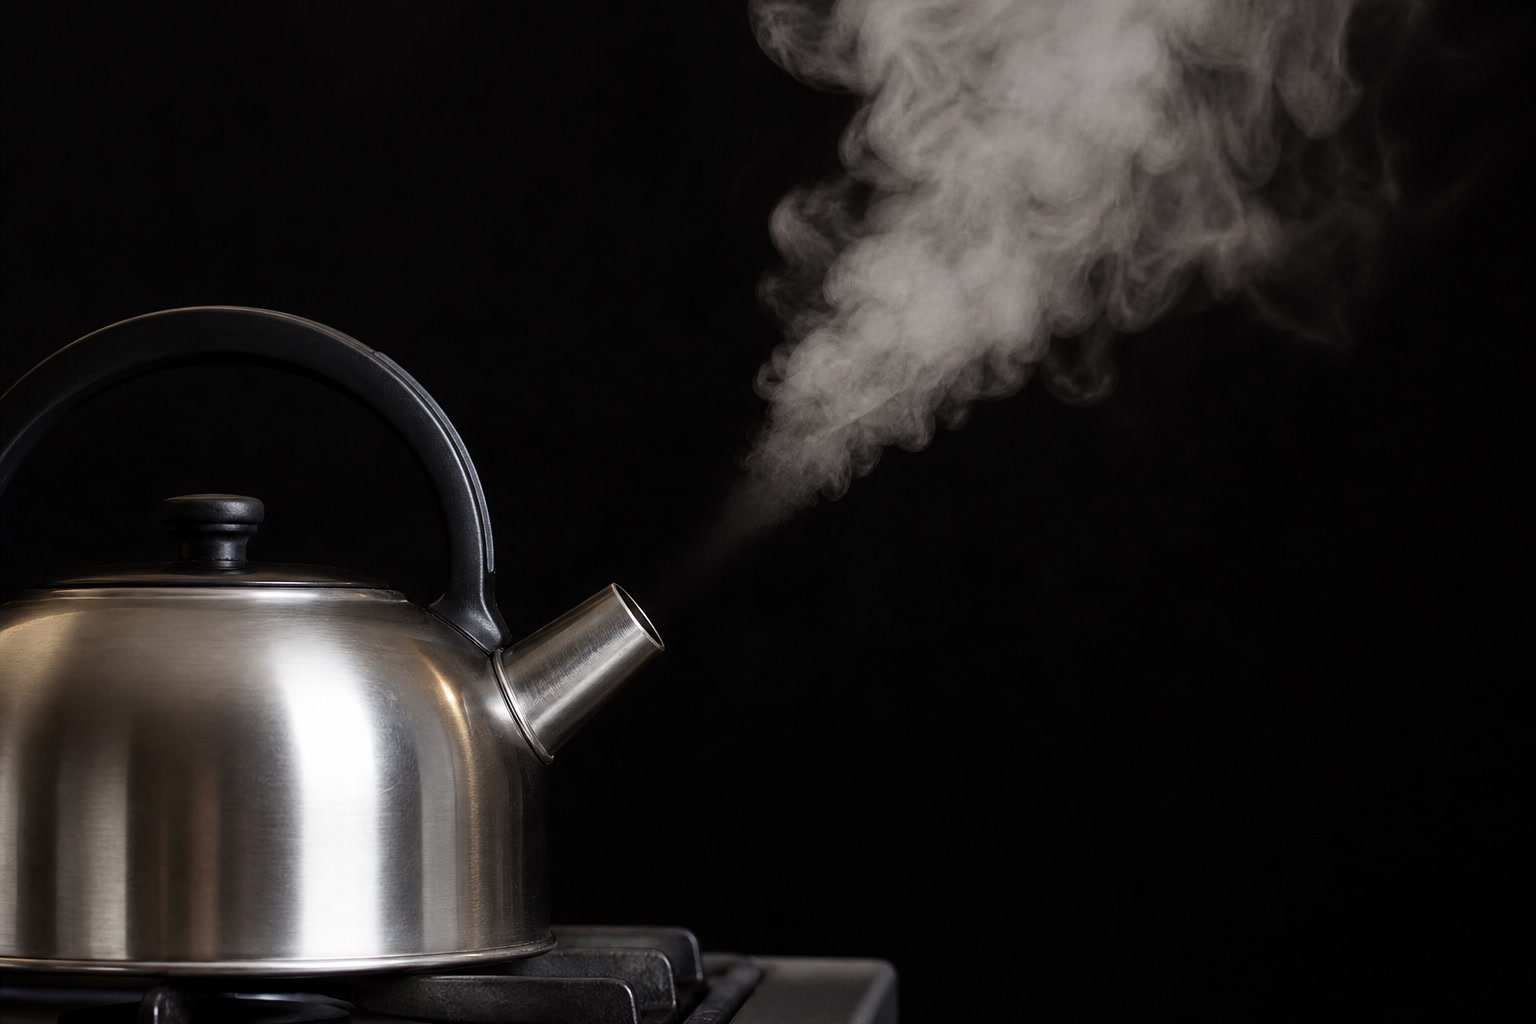
\includegraphics[width=0.55\linewidth]{images/book1/ai/g2-ice-water-steam-kettle.jpg}

{\small 水壶的秘密：就在壶嘴正上方，有一小段\emph{透明}的空隙，那里的水是看不见的气体——只有再往上，它才凝结成我们能看到的白色水汽。}
\end{omfigure}

\section{状态的变化}

\begin{definition}[熔化与凝固]\label{def:g2:ice-water-steam:meltfreeze}
当热量使固体的冰变为液体的水时，冰
\emph{熔化}\index{熔化}。当强冷使水由液体变为固体时，
水\emph{凝固}\index{凝固}。熔化与凝固是
同一两种状态之间相对的两扇门：热量推向一个方向，
低温推向另一个方向。
\end{definition}

\begin{definition}[蒸发与凝结]\label{def:g2:ice-water-steam:evapcond}
当热量使液体的水以气体形式飞入空气中时，水
\emph{蒸发}\index{蒸发}——水洼变小，
衣服变干。当水蒸气接触到冷的物体并变回
液体的小水滴时，它就\emph{凝结}\index{凝结}——
冷窗上的雾气，镜子上的雾。又是两扇
相对的门：热量使水进入气体状态，低温使它回到
液体状态。
\end{definition}

\begin{omfigure}
\begin{tikzpicture}[scale=0.85]
  \node[font=\small, draw, thick, omDef, minimum width=1.9cm,
    minimum height=0.85cm] (ice) at (0.8,0) {固体};
  \node[font=\small, draw, thick, omDef, minimum width=1.9cm,
    minimum height=0.85cm] (water) at (5.3,0) {液体};
  \node[font=\small, draw, thick, omDef, minimum width=1.9cm,
    minimum height=0.85cm] (steam) at (9.8,0) {气体};
  \draw[-Stealth, very thick, omThm] (1.85,0.28) -- (4.25,0.28);
  \node[above, font=\small, omThm] at (3.05,0.42) {热量：熔化};
  \draw[-Stealth, very thick, omDef] (4.25,-0.28) -- (1.85,-0.28);
  \node[below, font=\small, omDef] at (3.05,-0.42) {低温：凝固};
  \draw[-Stealth, very thick, omThm] (6.35,0.28) -- (8.75,0.28);
  \node[above, font=\small, omThm] at (7.55,0.42) {热量：蒸发};
  \draw[-Stealth, very thick, omDef] (8.75,-0.28) -- (6.35,-0.28);
  \node[below, font=\small, omDef] at (7.55,-0.42) {低温：凝结};
\end{tikzpicture}

{\small 状态的变化：热量总是推向右边，
低温总是推回左边。}
\end{omfigure}

\begin{example}[试试看：捉住看不见的水]\label{ex:g2:ice-water-steam:catch}
从冰箱里直接拿出一罐饮料或一只杯子，
用毛巾仔细擦干外面，然后放在桌上。在
你数到 $100$ 的时候，外面先变得雾蒙蒙，接着变湿——水滴
凭空出现！它们不是透过杯子渗出来的：
房间空气中看不见的水蒸气碰到了冷的杯壁，并
在上面凝结。你刚刚捉住了看不见的气体。
\end{example}

\begin{example}[呼气成雾]\label{ex:g2:ice-water-steam:breath}
你呼出的气体中总含有看不见的水蒸气。在温暖的日子里，它
仍然看不见。在寒冷的早晨，室外的冷空气
会立刻使它凝结成嘴前的一小团白雾——
同样的事情也会发生在冷窗上：你对着它呵气，
然后用手指在上面画画。
\end{example}

\begin{remark}[蒸汽与炉灶：注意安全]\label{rem:g2:ice-water-steam:safety}
沸腾的锅上方的水蒸气烫得很，比
水本身摸起来还要烫。千万不要把手伸进蒸汽里，揭锅盖时要朝远离自己的方向掀开，身边要有大人。
只要用到炉灶，状态变化
只供观察，不可用手去碰。
\end{remark}

\section{同一种水，周而复始}

\begin{example}[水洼变小了]\label{ex:g2:ice-water-steam:puddle}
雨过之后，操场上的一个水洼闪闪发亮。到了下午，
水洼变小了；到了第二天，它就不见了。
没有人喝它，它也没有渗进沥青地面，
是太阳的热量让它一滴一滴地蒸发，跑进了空气里。早上沿水洼画一条粉笔线，
午饭后再查看：水已经退到线的里面了。
\end{example}

\begin{example}[从海洋到雨水]\label{ex:g2:ice-water-steam:cycle}
蒸发掉的水，必定会在某处凝结。水从大海和水洼中
悄悄飞上天空，看不见；在高空那寒冷的空气里，
它凝结成形成云的小水滴；小水滴聚在一起，越长越重，落下来，就是雨！雨水注满水洼和大海，
循环又重新开始。
你杯子里的水，
已经往返过无数次，多得数也数不清。
\end{example}

\section{练习}

\begin{exercise}[$\star$]\label{exo:g2:ice-water-steam:1}
说出下列各物分别是哪种物态：固体、液体还是气体：
冰柱；\ 大海；\ 汤锅壶嘴正上方看不见的
水汽；\ 草上的霜；\ 雨？
\end{exercise}

\begin{exercise}[$\star$]\label{exo:g2:ice-water-steam:2}
说出下列各种状态变化：太阳下缩小的雪人；\ 水洼
消失；\ 浴室镜子上出现雾气；\ 池塘
冬天凝固成冰。
\end{exercise}

\begin{exercise}[$\star$]\label{exo:g2:ice-water-steam:3}
在状态变化图中，热量总是把物质推向哪一边：
推向固体还是气体？那么冷呢？
\end{exercise}

\begin{exercise}[$\star$]\label{exo:g2:ice-water-steam:4}
\cref{ex:g2:ice-water-steam:catch}中冷罐上的水珠——
是从玻璃里漏出来的吗？它们是从哪里来的？
\end{exercise}

\begin{exercise}[$\star$]\label{exo:g2:ice-water-steam:5}
为什么在寒冷的早晨能看见呼出的气，
而在温暖的日子里却看不见？请用\cref{def:g2:ice-water-steam:evapcond}中的术语回答。
\end{exercise}

\begin{exercise}[$\star$]\label{exo:g2:ice-water-steam:6}
湿衣服在太阳下比在阴凉处干得快。起作用的是哪种
状态变化？太阳又添了什么，让它干得更快？
\end{exercise}

\begin{exercise}[$\star$]\label{exo:g2:ice-water-steam:7}
沸腾的锅上方的蒸汽柱为什么很危险，
\cref{rem:g2:ice-water-steam:safety}中给出的安全规则是什么？
\end{exercise}

\begin{exercise}[$\star$]\label{exo:g2:ice-water-steam:8}
讲一讲一滴雨水的往返旅程：从大海出发，
最后回到大海，途中要用上“蒸发”和“凝结”这两个词。
\end{exercise}

\begin{exercise}[$\star\star$]\label{exo:g2:ice-water-steam:9}
锅嘴上有一段透明的空隙，白色的蒸汽柱
只在它的上方才开始出现。透明的空隙里是什么？
这说明气态的水具有什么特点？
\end{exercise}

\begin{exercise}[$\star\star$]\label{exo:g2:ice-water-steam:10}
尼诺把一杯水放在窗台上一个星期，水位
一天天下降，可是没有人喝它。他的猫被指控了。
替猫辩护：解释真正发生了什么，并想出一种方法，
证明水是\emph{跑进了空气中}，而不是进了猫的肚子里。
\end{exercise}
